\documentclass{article}
\usepackage[utf8]{inputenc}
\usepackage{graphicx}
\usepackage{multirow}

\usepackage{lipsum}
\usepackage{listings}
\usepackage{xcolor}
\lstset { %
    language=C++,
    backgroundcolor=\color{black!5}, % set backgroundcolor
    basicstyle=\footnotesize,% basic font setting
}

\title{CMSE 822 Final Project }
\author{Carolyn Wendeln $\&$ Gabe Appleton}

\date{\today}

\begin{document}

\maketitle

\section{Abstract}
\section{Introduction}

Modern astrophysical research has become increasingly dominated by large scale, multi-dimensional simulations.
Phenomena such as supernovae core collapse, coronal mass ejections, or neutron star mergers all rely on multi-scale simulations.
These simulations can span orders of magnitude in scale separation, yet these vast scales are required to resolve the key underlying physics involved.
Although these large scale simulations have become a necessity, they often require an ever-increasing amount of computational resources.

One key feature that most of these astrophysical phenomena have in common is that they are often coupled to hyperbolic partial differential equations (PDEs).
Equations such as Euler, Cauchy, or Navier–Stokes are often used for simulating astrophysical plasmas.
These simulations often call for techniques such as adaptive mesh refinement (AMR) and high order finite difference or finite volume methods.

For this research project, I will be investigating second and fourth order discretization of hyperbolic PDEs.
In particular, I will look at the two dimensional form of the advection equation, viscous Burgers' equation, and inviscid Burgers' equation.
This work will focus on these equations over a periodic domain on a uniform mesh grid using finite difference methods.

The goal of this research project is to understand the underlying issues surrounding hyperbolic solvers for fluid equations.
I will investigate various optimization techniques for a single node.
My work will begin with parallelization using OpenMP 4.5 or 5.0. to target both CPUs and GPUs.
After parallelisation, I will employ other techniques such as cache blocking to see the effects of strong and weak scaling.
Once I believe I have achieved optimal performance using OpenMP, I will try to implement similar techniques using Kokkos.

Kokkos is an open source c++ performance portability programming model that has recently been coupled with Athena++ to create K-Athena.
Athena++ is a magnetohydrodynamics CUP code that is based on MPI+OpenMP.
K-Athena utilizes MPI for inter-node parallelism, hence my project here will focus solely on optimization for a single node.
Likewise Kokkos is compatible with optimization techniques which target both CPUs and GPUs.
K-Athena will become a key component to my own thesis, so this research project serves as a fantastic stepping stone to my future research studying astrophysical phenomena using AMR and finite volume methods.

\section{Methodology}

For this research project, we look to solve and parallalize three PDEs. The first is the linear advection equation, which can be described as 

\begin{equation}
 \frac{\partial a}{\partial t} + u \frac{\partial a}{\partial x} = 0
\end{equation}

where $a(x,t)$ is a scalar quantity and $u$ is the velocity at which it is advected. For our research project, we chose to make $a(x,t)$ a Gaussian function of the form 

\begin{equation}
a(x,t) = a_0(t) e^{- 50 (x - 0.5)^2 }
\end{equation}

To solve this PDE, we use a finite-difference discretization in which the domain is divided into a sequence of points where we store the solution. We then solve this PDE numerically by discretizing the solution at these points.





\begin{figure}[h]
\centering
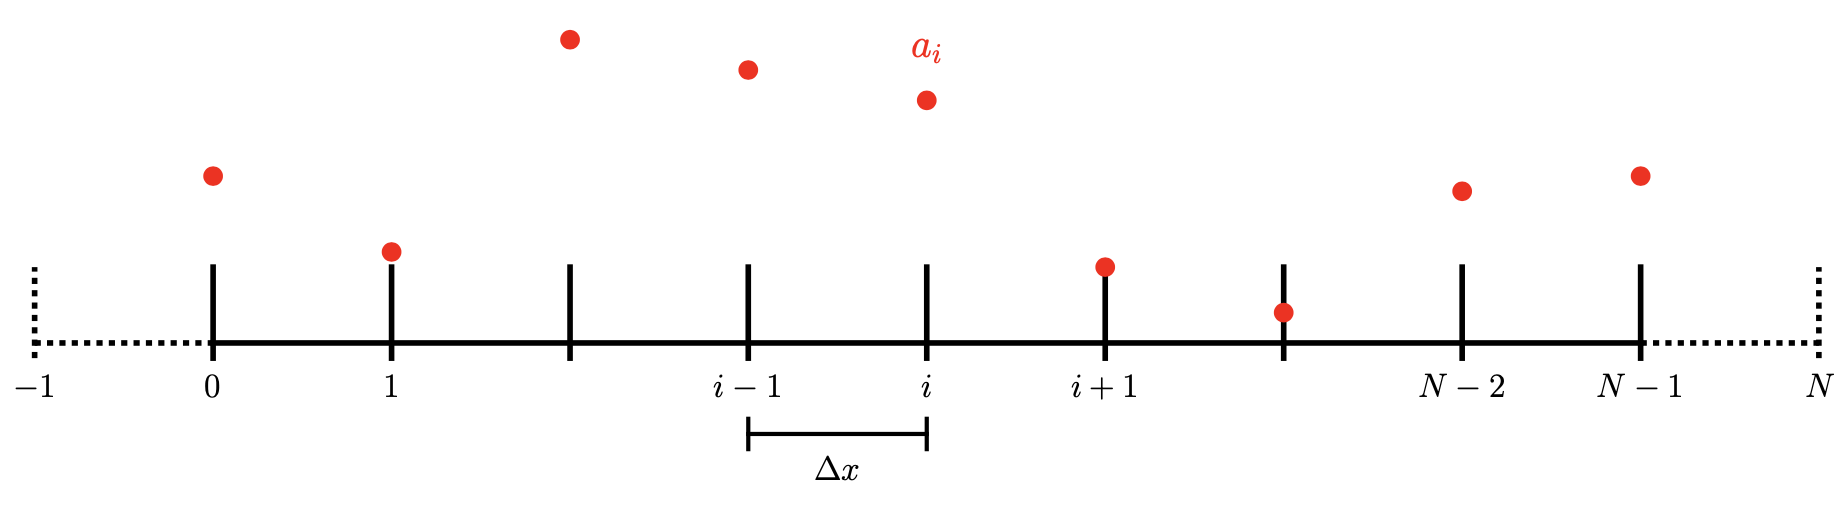
\includegraphics[width=1.0\textwidth]{Finite_Difference_Grid.png}
\caption{A simple finite-difference grid (courtesy of \cite{zingale_2020}). The solution is stored at each of the labeled points. The dotted lines show the ghost points used to extend our grid past the physical boundaries to accommodate boundary conditions. In our instance, we assume a periodic domain, so the points $0$ and $N-1$ are the same physical point in space.}
\label{Finite_Difference_Grid}
\end{figure}

Let the index $i$ denote the point's location, and $a_i$ denote the discrete value of $a(x)$ at point $i$. Figure ~\ref{Finite_Difference_Grid} shows the grid. To discretize in time, we denote the time-level with a superscrip $n$, such that $a_i^n = a(x_i, t_n)$. For a fixed $\Delta t$, a time level $n$ corresponds to a time of $t = n \Delta t$. A simple first-order accurate centered-difference discretization is then

\begin{equation}
 \frac{a_i^{n+1} - a_i^n}{\Delta t} + u \frac{a_{i+1}^n - a_{i-1}^n}{2 \Delta x}  = 0
\end{equation}

This is a forward-time, centered-space explicit method, since the new solution, $a_i^{n+1}$, depends only on information at the old time level, $n$. When implimented into \texttt{C++}, we are itterating through time steps $n$ and displacment steps $i$ to solve for $a_i^{n+1} $

The second equation we wish to investigate is Inviscid Burgers’ equation. This equation is a nonlinear hyperbolic equation, and given as:

\begin{equation}
 \frac{\partial a}{\partial t} + a \frac{\partial a}{\partial x} = 0
\end{equation}

Here $a(x,t)$ is both the quantity being advected and the speed at which it is moving. The centered-difference discretization for Inviscid Burgers' equation is then

\begin{equation}
 \frac{a_i^{n+1} - a_i^n}{\Delta t} +  a_i^n ( \frac{a_{i+1}^n - a_{i-1}^n}{2 \Delta x} ) = 0
\end{equation}

The third and final equation we wish to investigate is Viscous Burgers' equation

\begin{equation}
 \frac{\partial a}{\partial t} + a \frac{\partial a}{\partial x} = \nu \frac{\partial ^2 a}{\partial x^2} 
\end{equation}

Here $\nu$ is the viscosity. The centered-difference discretization for Viscous Burgers' equation is then

\begin{equation}
 \frac{a_i^{n+1} - a_i^n}{\Delta t} + a_i^n ( \frac{a_{i+1}^n - a_{i-1}^n}{2 \Delta x} ) = \nu (\frac{a_{i+1}^n - 2a_i^n - a_{i-1}^n}{{\Delta x}^2})
\end{equation}

For this research project we aim to parallize and time the speed for our code to run through the bulk of our data (excluding the special boundary conditions to main periodicy). For example, the 1D Advection would appear as:

\begin{lstlisting}
double start = omp_get_wtime();

#pragma omp parallel for num_threads(thrd_cnt)

for(int t=0; t<n; ++t)
{
	for(int i=1; i<(N-2); ++i)
   	{
   		a_write[i] = a_read[i] - 
   		(((u * delta_t) / (2 * delta_x)) 
   		* (a_read[i+1] - a_read[i-1]));
  	}

	double end = omp_get_wtime();
	double time_taken = end-start;
	
	loop_time[t] = time_taken;
}	
\end{lstlisting}



\begin{center}
\begin{tabular}{ |c|c|c|c|c|c| } 
\hline
 & Scaling & Schedule & N & n & t \\
\hline
\multirow{8}{4em}{2D Advection} & \multirow{4}{4em}{strong}& none & 32 - 2,048 & 10,00 & 1 - 8 \\ 
& & static & 32 - 2,048 & 10,00 & 1 - 8 \\
& & dynamic & 32 - 2,048 & 10,00 & 1 - 8 \\ 
&  & guided & 32 - 2,048 & 10,00 & 1 - 8 \\ 
\cline{2-2} % add this

& \multirow{4}{4em}{weak}& cell3 & cell 4 & cell 5 & cell 6 \\ 
& & cell6 & cell 7 & cell 8 & cell 9\\ 
& & cell6 & cell 7 & cell 8 & cell 9\\ 
&  & cell9 & cell 10 & cell 11& cell10 \\ 
\hline
\end{tabular}
\end{center}

For 2D Advection, 2D Inviscid Burgers, and 2D Viscous Burgers we wish to look at strong and weak scaling, while incorportationg cache blocking by loop scheduling. A detailed summary can be found in Table 




\section{Discussion}
\section{Conclusion}
\section{Acknowledgments}

C. W. would like to thank Dr. Andrew Christlieb for his invaluable knowlege on numerical solutions to PDEs.







 \bibliography{Final_Report_Bibliography} 
\bibliographystyle{apalike}

\end{document}